%no borrar PREAMBULO
\documentclass[12pt]{article}

\usepackage[top=3.5 cm, bottom=2.5  cm, left=3 cm, right=3 cm]{geometry}
\usepackage{fancyhdr}
\pagestyle{fancy}

\usepackage[hidelinks]{hyperref} %esta opción saca las cajas de colores de los hiperlinks

\fancyfoot[C]{\thepage }  %numera las páginas

\usepackage[utf8]{inputenc}

\usepackage{amsmath,amsfonts,amssymb}
\usepackage{xcolor}
\usepackage{fancyvrb}
\newcommand\verbbf[1]{\textcolor[rgb]{0,0,1}}%comando para colorear el texto en verbatim

%\linespread{1} %por si queremos achicar el espacio entre lineas

\usepackage{tabularx,booktabs}
\usepackage{graphicx}
\usepackage{float} %para que las figuras puedan ponerse en cualquier lado

\usepackage{svg} % Figuras en .svg

\usepackage{subcaption}
\usepackage{layout}
\usepackage{multicol}  %para escribir en columnnas 
\usepackage{float}
\usepackage{textcomp}
\usepackage{natbib}
\usepackage{tikz}
\usepackage{multirow} %para cambiar el alto de una fila en una tabla
\tikzset{
  connect/.style = { dashed, gray }
}
\usepackage{pgfplots}
\pgfplotsset{compat=1.8}
\usepackage[english ,spanish]{babel}
\usepackage{latexsym}
\usepackage{verbatim}

%\usepackage{alltt}
\usepackage{indentfirst}

\usepackage{fancybox, calc} 

\usepackage[flushmargin]{footmisc} %para alinear las notas de página

\usepackage{url}
\usepackage{advdate}
\usepackage{wrapfig}
\usepackage{amsthm}
\usepackage[inline]{enumitem} %para hacer listas en una linea, los mismos comandos con *
\newtheorem*{myteo}{Teorema} % la * es para no numerarlos
\newtheorem*{myexample}{Ejemplo}
\newtheorem*{myprop}{Proposición}
\newtheorem*{mylem}{Lema}
\theoremstyle{definition}
\newtheorem*{mydef}{Definición}
\newtheorem{ejer}{Ejercicio}
\newtheorem*{mydefs}{Definiciones}
%\theoremstyle{remark}
\newtheorem*{myobs}{Observación}
\newtheorem*{remark}{Importante}

\renewcommand{\baselinestretch}{1}  %interlineado

\addto\captionsspanish{%
  \renewcommand{\figurename}{Figura}%
}

\newcommand\myText[1]{\text{\scriptsize\tabular[t]{@{}l@{}}#1\endtabular}}
\addto\captionsspanish{%
  \renewcommand{\tablename}{Tabla}%
}

\def \ds {\displaystyle} %define un comando abreviado  
\def\com{“R”}

\usepackage{hyperref}%para referencias de internet con link!
\newcommand*{\fullref}[1]{\hyperref[{#1}]{ \nameref*{#1}}}
%comando \fullref para que ademas del número de capitulo, sección etc. escriba el título del capitulo, sección o lo que sea a lo que estamos haciendo referencia

\newcommand\comentario[1]{\textcolor{red}{#1}}%comentarios en el pdf

\interfootnotelinepenalty=10000 %previene que se pasen a otra página las notas de pie
\raggedbottom 
\addtolength{\topskip}{0pt plus 10pt}
\addtolength{\footnotesep}{0.1mm}

\VerbatimFootnotes%para poder usar Verbatim en las notas de pie
\newcommand{\grad}{\hspace{-2mm}$\phantom{a}^{\circ}$} % Símbolo de grado

\usepackage{listings} % Para escribir código
\usepackage{xcolor}
\usepackage{amsmath} % Para recuadrar ecuaciones con \boxed
\usepackage{graphicx} % Para uso de figuras
\usepackage{svg} % Figuras en .svg
\usepackage{float} % Para ubicar una figura/tabla de manera forzada usando [H]
\definecolor{codegreen}{rgb}{0,0.6,0}
\definecolor{codegray}{rgb}{0.5,0.5,0.5}
\definecolor{codepurple}{rgb}{0.58,0,0.82}
\definecolor{backcolour}{rgb}{0.95,0.95,0.92}

\def\mcolor#1#{\@mcolor{#1}}
\def\@mcolor#1#2#3{\protect\leavevmode\color#1{#2}#3\color{black}}

\begin{document}

\fancyhf{}
\pagestyle{fancy}
\lhead{Departamento de Matem\'{a}tica\\Universidad Nacional del Comahue}
\rhead{Matem\'{a}tica 1\\ Licenciatura en Ciencias Biol\'{o}gicas}

%HASTA ACA 

\begin{centering}
\Large{\textbf{Trabajo Práctico N° 1}}\\
\large{\textbf{Soluciones de ejercicios seleccionados}}\\

\small{\textbf{Nociones básicas de conjuntos. Relaciones y operaciones}}\\
\end{centering}
\vspace{1cm}
\noindent
En este documento ofreceremos las soluciones de algunos ejercicios y problemas seleccionados de este Trabajo Práctico con explicaciones que permitan seguir el razonamiento para su resolución. Como la numeración de los ejercicios de las distintas versiones del TP pueden variar, incluimos antes de la solución, el ejercicio que se resolverá.

\begin{enumerate}
%1
\item \textbf{Ejercicio 1:} Escribir los conjuntos siguientes por comprensión, explicitando claramente el referencial. Hacerlo lo más formalmente que puedas (no es obligatorio el uso de símbolos, sí la precisión):
\begin{multicols}{2}
$A = \{ 0, 1, -1, 2, -2, 3, -3 \}$ \\
$ B = \{ l, e, c, v, a \}$  \\
$C = \{ 1, 3, 5, 7, 9, 11, 13, 15, 17, 19 \}$\\
$D = \{1, 2, 3, 4, 6, 12 \}$   
\end{multicols}

\vspace{0.5cm}
\noindent
\textbf{Solución} \\
En estos ejemplos es importante primero reconocer el conjunto referencial, y luego establecer, dentro de ese conjunto referencial, cuál es la propiedad o la condición que cumplen los elementos que constituyen el conjunto.\\
\begin{itemize*}
\item  El conjunto está formado por números enteros (éste será el referencial) desde $-3$ hasta $3$ inlcuyendo estos números. Simbólicamente, este conjunto se escribe:\\
$A = \{ x \in \mathbb{Z} /  -3 \leq x \leq 3\}$ \\
\item El conjunto está formado letras, entonces el referencial será el conjunto de letras del abecedario. Las letras de este conjunto son las que forman la palabra  \textit{clave} (o clavel, o cualquier otra combinación). Simbólicamente, este conjunto se escribe:\\
$B = \{ x \in\text{ al abecedario}/ \text{ x es una letra de la palabra \textit{clave}}\}$ \\
\item El conjunto está formado por números naturales (referencial). Los números que constituyen este conjunto son impares y menores que $20$ o menores o iguales que $19$. Simbólicamente, este conjunto se escribe:\\
$C = \{ x \in \mathbb{N} /  x \text{ es impar y }  x \leq 19\}$ \\
\item El conjunto está formado por números naturales (referencial). Los números que constituyen este conjunto son divisores de $12$. Simbólicamente, este conjunto se escribe:\\
$C = \{ x \in \mathbb{N} /  x \text{ es divisor de } 12\}$ \\
\end{itemize*}

%4 
\item  \textbf{Ejercicio 4:} Dados los siguientes conjuntos: $A= \{ 1,2,3,4 \}$, $B= \{ 2,4,6,8 \}$, $C = \{ 3,4,5,6 \}$  dentro del referencial $R = \{x \in \mathbb{N} /  x \leq 10 \}$ , hallar:
\begin{table}[ H]
\begin{center} 
\begin{tabular} { c c c c c c c c c }
 $A \cup B$ &&  $A \cup C$ &&  $B \cup B$ && $A \cap B$ && $A \cap C$ \\ \\
 $A \cap B \cap C$ &&  $A  - B $ &&  $C - A$ && $B - B$ && $ \overline A$ \\ \\
 $ \overline {A \cap B}$ &&  $ \overline {A \cup B}$ &&  $ \overline {A -B}$ && $ \overline {A \cup B \cup C}$ && $ \overline B$ \end{tabular} 
\end{center} 
\end{table}
%\vspace{0.5cm}
\noindent
\textbf{Solución} \\
Para hacer esto ayuda mucho graficar los conjuntos $A$, $B$ y $C$ dentro del referencial y ubicar los elementos en las regiones correspondientes. Para encontrar la solución de cada ítem pueden sombrear las zonas correspondientes y ver qué elementos están en ellas.\\
 \begin{center} 
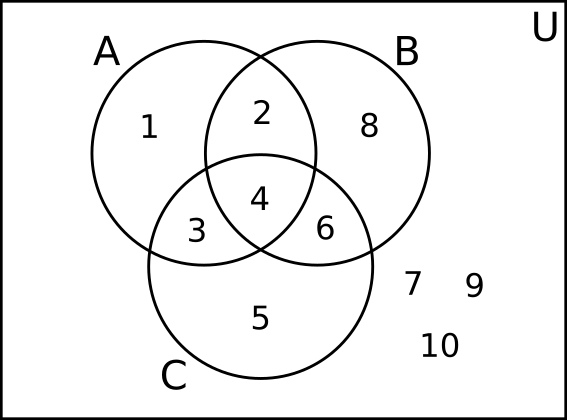
\includegraphics[width=0.5\textwidth]{tp_1_sol_f1.png} 
\end{center}
La \textbf{unión} de los conjuntos $A$ y $B$ es un nuevo conjunto que reúne los elementos de $A$ y los de $B$, comunes y no comunes:\\
\begin{itemize*}
\item  $A \cup B = \{ 1, 2, 3, 4, 6, 8 \}$ \\
\item  $A \cup C = \{ 1, 2, 3, 4, 5,  6 \}$\\  
 \item $B \cup B = B$ 
\end{itemize*}

\noindent
La  \textbf{intersección} de los conjuntos $A$ y $B$ es un nuevo conjunto que reúne solo los elementos comunes a $A$ y a $B$:\\
\begin{itemize*}
\item  $A \cap B= \{2, 4 \}$ \\
\item  $A \cap C= \{3, 4 \}$ \\
\item  $A \cap B \cap C= \{4 \}$ 
\end{itemize*}

\noindent
La  \textbf{diferencia} de los conjuntos $A$ y $B$ es un nuevo conjunto que reúne los elementos de $A$  excluyendo los que tiene en común con $B$:\\
\begin{itemize*}
\item  $A - B= \{1, 3 \}$ \\
\item  $C - A= \{5, 6 \}$ \\
\item  $B - B \cap C= \{ \} =\varnothing $ 
\end{itemize*}

\noindent
El \textbf{complemento} de un conjunto es un nuevo conjunto que reúne a todos los elementos del referencial que no pertenecen a ese conjunto. Así, el complemento de $A$ será el conjunto de los elementos del referencial que no pertenecen a $A$ y el complemento de la intersección de $A$ y $B$ sera el conjunto de los elementos del referencial que no pertenecen a esa intersección (es decir, todos los elementos del referencial que no son comunes a $A$ y $B$:\\
\begin{itemize*}
\item $ \overline {A}= \{5, 6, 7, 8, 9, 10\}$ \\ 
\item $ \overline {A \cap B}= \{1, 3, 5, 6, 7, 8, 9, 10\}$ \\
\item $ \overline {A \cup B}= \{5, 7, 9, 10\}$  \\
\item $ \overline {A - B}= \{2, 4, 5, 6, 7, 8, 9, 10\}$ \\
\item $ \overline {A \cup B \cup C}= \{7, 9, 10\}$ \\
\item $ \overline {B}= \{1, 3, 5, 7, 9, 10\}$ 
\end{itemize*}\\

%5
\item   \textbf{Ejercicio 5:} Considerar los siguientes conjuntos de números naturales: \\
$U =  \{x \in \mathbb{N} / x  \text{ es menor que 10} \}$, \\
$A =  \{x \in \mathbb{N} / x  \text{ es un número primo y } x \leq 7 \}$\\
$B =  \{x \in \mathbb{N} / x  \text{ es un número par y }  x \leq 7 \}$\\

Determinar:
\begin{table}[ H]
\begin{center} 
\begin{tabular} { c c c c c c c c c c c c c c c }
 $\overline A$ &&  $\overline B$ &&  $A \cap \overline B$ && $\overline A \cup  \overline B$ && $B \cup \overline B$ &&
 $\overline B \cap A$ &&  $\overline B \cap U$ &&  $\overline {A \cup B}$ 
 \end{tabular} 
\end{center} 
\end{table}

%\vspace{0.5cm}
\noindent
\textbf{Solución} \\
El referencial es el conjunto $U =  \{x \in \mathbb{N} / x  \text{ es menor que 10} \} =\{1, 2, 3, 4, 5, 6, 7, 8, 9\}$. Primero mostramos un gráfico en el que hemos representado los conjuntos:
 \begin{center} 
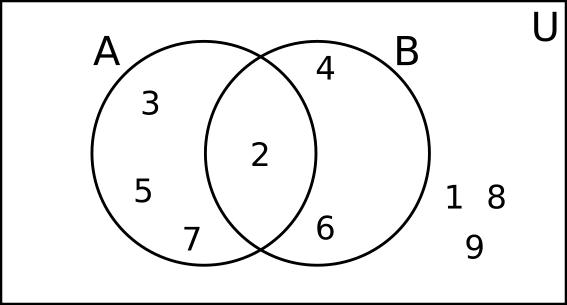
\includegraphics[width=0.5\textwidth]{tp_1_sol_f2.png} 
\end{center}
Entonces: \\
\begin{itemize*}
\item $ \overline {A}= \{1,4, 6, 8, 9\}$ \\ 
\item $ \overline {B}= \{1,3, 5, 7, 8, 9\}$ \\ 
\item $ A \cap \overline {B}= \{3, 5, 7\}$ \\
\item $ \overline {A} \cup \overline {B}= \{1,3,4, 5, 6, 7, 8, 9 \}$  \\
\item $ B \cup \overline {B}= U$ (es el referencial)\\
\item $ \overline {B} \cap U =\overline {B}$ \\
\item $ \overline {B} \cap A = \{3, 5, 7\}$ (igual al tercer ítem porque la intersección cumple con la propiedad conmutativa\\
\item $ \overline {B} \cap U= \overline {B} $ \\
\item $ \overline {A \cup B}= \{1, 8, 9\}$ 
\end{itemize*}\\

%6
\item\textbf{Ejercicio 6:}  Escribir una operación entre los conjuntos $A$, $B$ y $C$ que dé por resultado la zona sombreada en las figuras siguientes.\\
\textbf{Solución} \\
Hay muchas formas de expresar las regiones sombreadas con operaciones entre conjuntos. Les proponemos una para cada una, pero es posible que alguien encuentre alguna que, aunque se exprese de forma distinta, son equivalentes.
 \begin{center} 
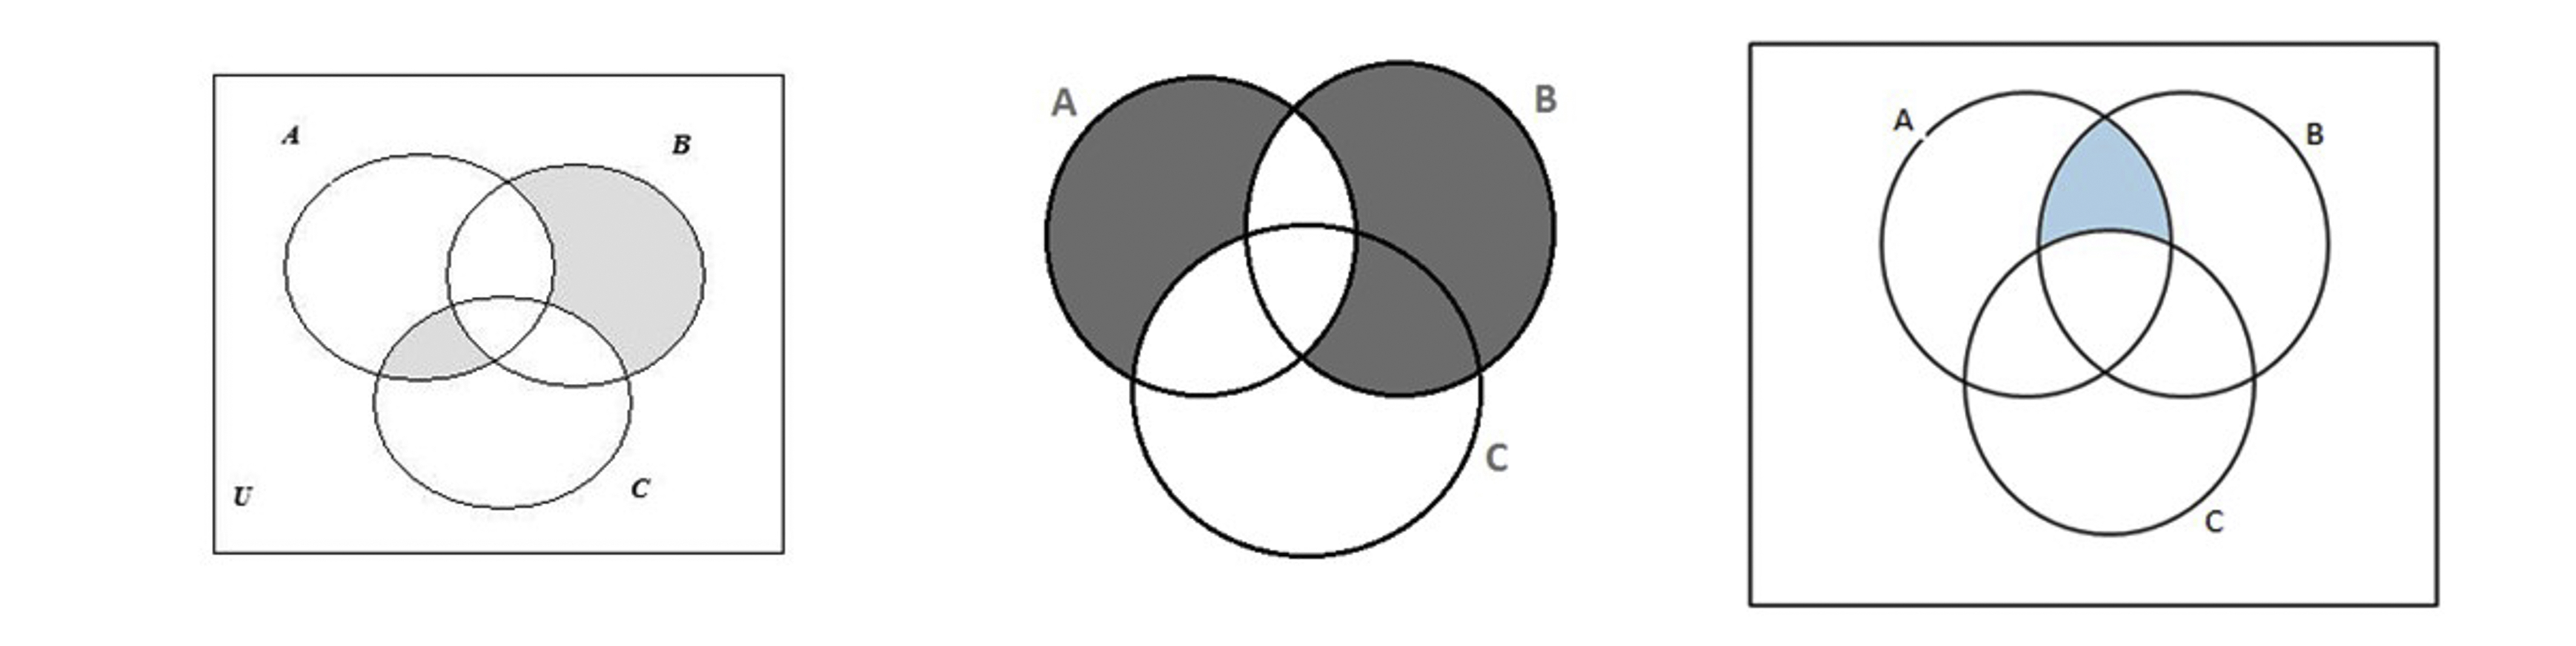
\includegraphics[width=1\textwidth]{tp_1_sol_f3.jpg} 
\end{center}

\begin{table}[H]
\begin{center} 
\begin{tabular} { c c c c }
$\left[ B- (A\cup C) \right] \cup \left[(A \cap C) - B \right]$ & $\left[ A - (B \cup C) \right] \cup (B-A)$ &&  $(A \cap B) - C$
  \end{tabular} 
\end{center} 
\end{table}
 
\begin{center} 
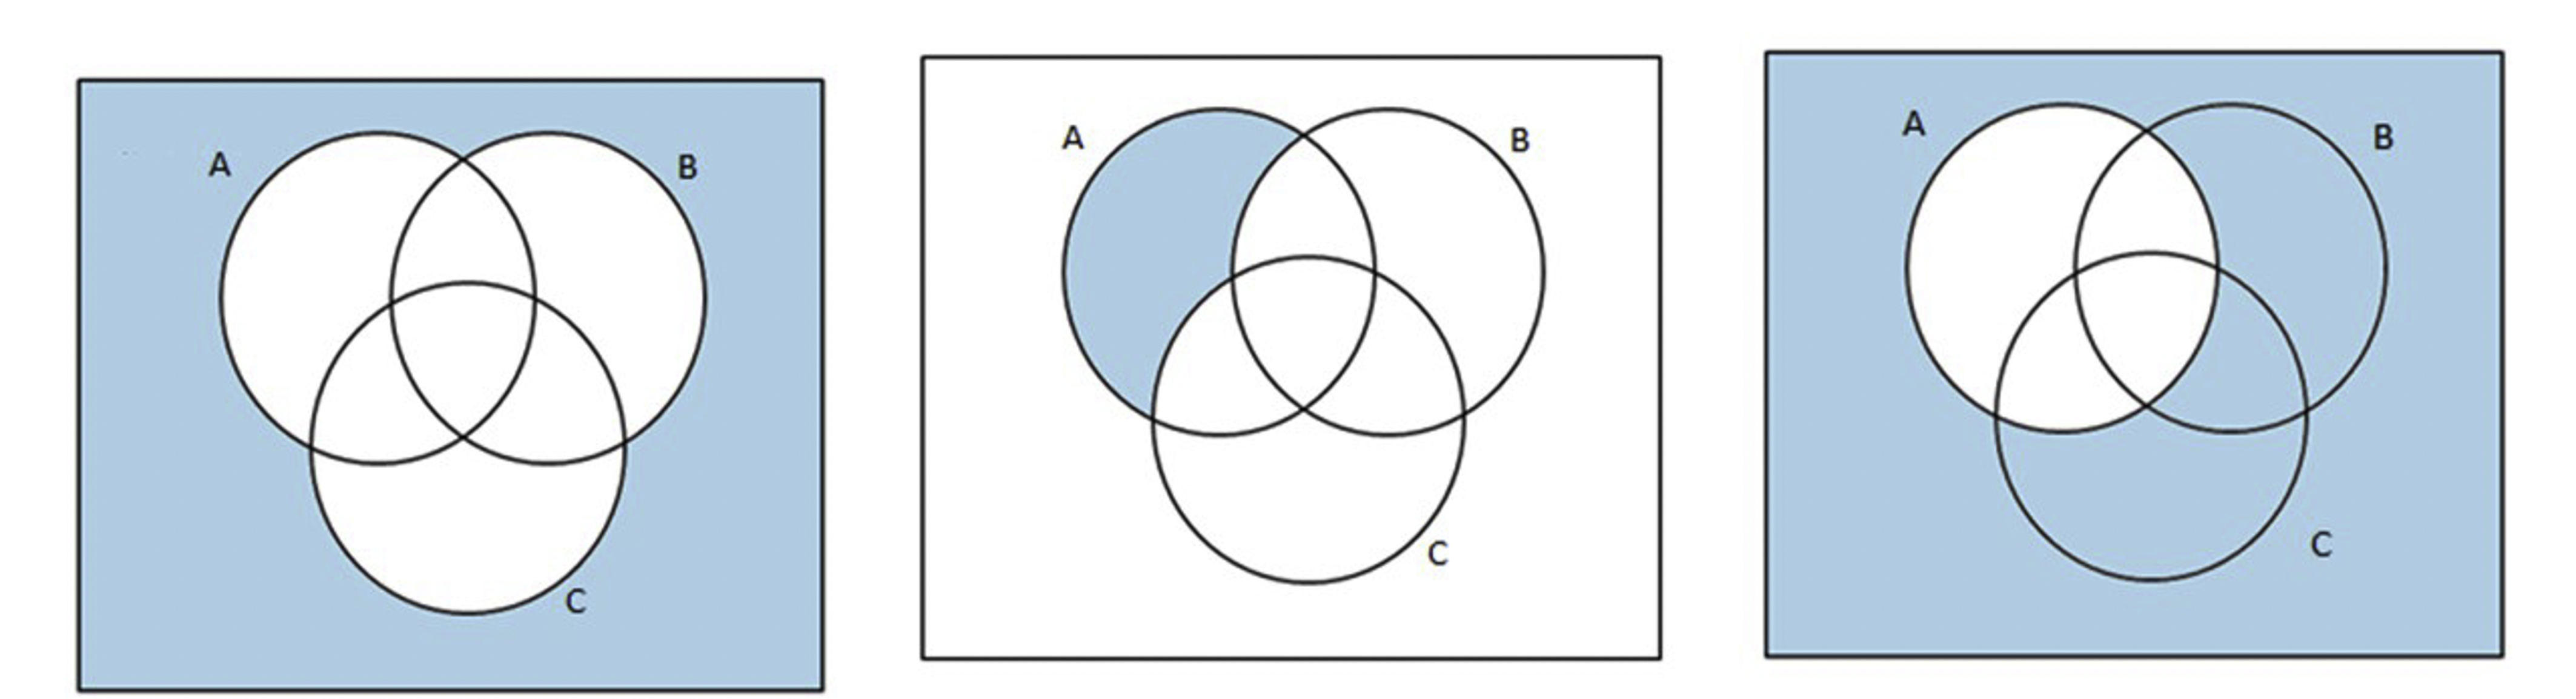
\includegraphics[width=1\textwidth]{tp_1_sol_f4.jpg} 
\end{center}

\begin{table}[H]
\begin{center} 
\begin{tabular} { c c c c c c c c c c c c c c c c }
$ \overline { A \cup B \cup C }$ &&&&& &  $A - (B \cup C)$ & & &&&&&& &  $\overline {A}$
  \end{tabular} 
\end{center} 
\end{table}
 

%fin listado de ejercicios
\end{enumerate}


\end{document}
